\section{Introduction}~\label{intro}
Robots operating in real-world environments often have incomplete or unreliable information about the current state of the world. Perception errors~\cite{kaipa2016addressing}, execution failures~\cite{kaelbling1998planning}, and unexpected environmental changes~\cite{kurniawati2016online} can leave multiple possible interpretations of the current situation. If a robot continues execution without resolving such ambiguity, it may make incorrect decisions and eventually fail the task. External information from an expert can help resolve this uncertainty~\cite{dragan2013legibility, goodrich2008human}. However, requesting external information whenever uncertainty arises is also undesirable, particularly in long-horizon tasks where frequent interaction can incur substantial costs in terms of time and workload~\cite{chen2014human}. The robot must therefore determine when external information is necessary and what information should be requested.


Recent uncertainty-aware systems address this problem by selectively requesting external feedback during task execution~\cite{ren2023robots, liang2024introspective, mullen2025lbap}. A common approach is to trigger a query based on the confidence of an action prediction or to select a query according to its expected effect on task reward. These approaches provide useful mechanisms for deciding whether additional information is needed, but the resulting query decision is often tied to action selection or task-level utility. In contrast, we focus directly on uncertainty about the current symbolic state. Rather than asking an external expert to choose an action or resolve the planning problem, the robot asks for a specific state fact and remains responsible for subsequent planning and execution.


We present a method that maintains a weighted belief over alternative symbolic world states throughout task execution. We formulate decision making as a partially observable Markov decision process (POMDP)~\cite{kaelbling1998planning} and represent task knowledge using a STRIPS-style symbolic model~\cite{davis1993knowledge,fikes1971strips}. After each action and observation, the belief is updated according to the available evidence. The uncertainty of this belief is then used to determine whether external information is required. When a query is triggered, the robot selects the symbolic state fact expected to reduce uncertainty the most and asks an external expert to verify it. The response removes inconsistent hypotheses and refines the belief used for subsequent planning.


\begin{figure}[t]
\captionsetup{skip=0pt}
\centering
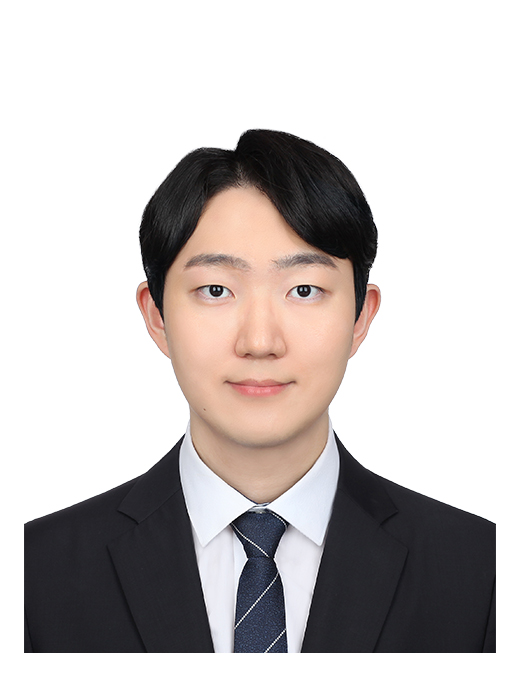
\includegraphics[width=0.5\linewidth]{figures/intro_and_method/fig_intro.jpg}
\caption{Overview of the proposed framework. A centralized knowledge base connects sensing, planning, feedback management, and user interaction. The robot maintains uncertainty over symbolic world hypotheses and uses this uncertainty to decide whether to continue autonomous execution or request state-level feedback.}
\label{fig:intro}
\end{figure}


As illustrated in Fig.~\ref{fig:intro}, the framework connects sensing, planning, feedback management, and external feedback through a centralized knowledge base. The belief over symbolic hypotheses is updated as new observations become available. If the belief remains insufficiently resolved, the framework requests verification of an uncertain state fact and incorporates the response into the belief before continuing execution. This allows the framework to separately determine when additional information is necessary and which information should be acquired.


We evaluate the proposed method in tomato harvesting and waste sorting, which exhibit different forms of state uncertainty. We first use an oracle feedback source to quantitatively analyze the effects of query timing and query content and to compare the proposed method with conformal-prediction-based and reward-based strategies. We then extend the evaluation to more realistic feedback sources, including a VLM and human participants, together with the KnowNo baseline, to examine whether the observed trends remain consistent across different sources of external feedback. Finally, we report qualitative findings from interviews with five participants to characterize how the proposed querying behavior is perceived during interaction.

The main contributions of this work are as follows:

\begin{itemize}

\item We determine when to query based on uncertainty in the current symbolic state and show that appropriate query timing improves task success.

\item We prioritize state information that is expected to reduce uncertainty and show that informative query selection reduces the number of required queries.

\item We compare the proposed method with conformal-prediction-based and reward-based strategies and show that it achieves higher task success without substantially increasing the number of queries.


\end{itemize}
